\documentclass{neu_handout}
\usepackage{url}
\usepackage{amssymb}
\usepackage{amsmath}
\usepackage{marvosym}
\usepackage{graphicx}
\graphicspath{ {images/} }
\everymath{\displaystyle}

% Professor/Course information
\title{Update 1}
\author{Emily Dutile, Vyshaal Narayanam, Xiwen Song, Yu Tian}
\date{November 2017}
\course{CS6220}{Data Mining Techniques}

\begin{document}

\section*{1. Problem Statement and Background}
As stated in our proposal, we look to address the following two questions:

(1) What topics are discovered frequently in reviews and do they correlate to a positive or negative review? What should a restaurant focus on to make their rating/reviews better?

(2) What neighborhoods in Pittsburgh have the best cuisine selection? Are there some areas that are more authentic, trendy, upscale or divey than others? Based upon reviews of the top restaurants in Pittsburgh, can we recommend restaurants to a user?

\section*{2. Methods}

\subsection*{2.1 Data Collection and Transformation}
With the Yelp Open Dataset\footnote{\url{https://www.yelp.com/dataset}} consisting of 4.7 million reviews, 156,000 business, and 12 metropolitan areas, we needed to filter out a signification amount of data and perform some further exploration in order to set potential thresholds to either include or exclude some data.\\
To get started, we created local databases and imported the given SQL file using MySQL Server and PyCharm in our development environment. This allowed us to begin writing queries in order to better understand our dataset and possibly explore other questions. From here, we narrowed down and verified what attributes we wanted to use in order to help answer our original questions.  Using Jupyter Notebooks, we extracted the data from SQL queries and stored them in two Pandas DataFrames, to then be able to create some basic visualizations and calculations in order to better filter, preprocess, and understand our data.\footnote{GitHub: \url{https://github.com/emily-jean/yelp-data-mining}}\\

\begin{center}
Yelp Data Schema\\
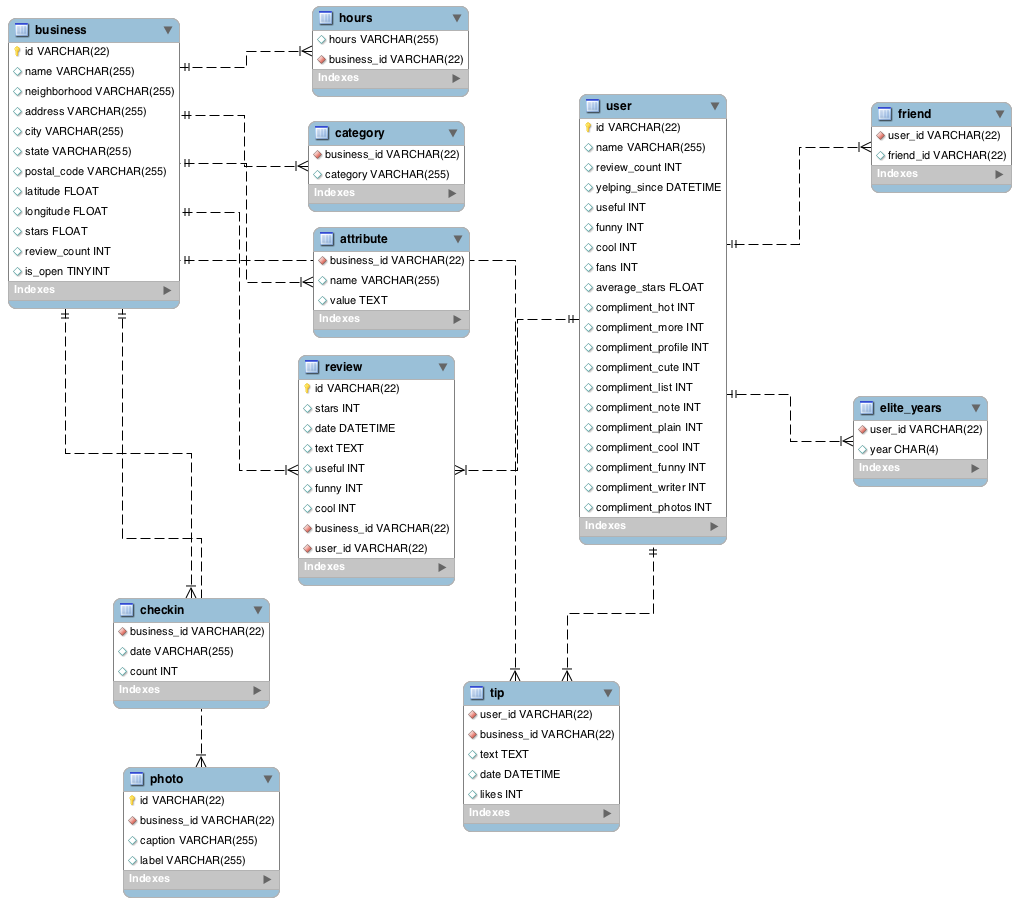
\includegraphics[width=75mm,scale=0.4]{schema}\\
\end{center}

\subsection*{2.2 Exploratory Analysis}

   Since Boston didn't appear to be in the data set, we first performed some analysis on what other city we'd like to look at in order to perform clustering and recommendation on. We extracted some sample data with sql queries and made visualizations of the data statistics.
   
\begin{center}
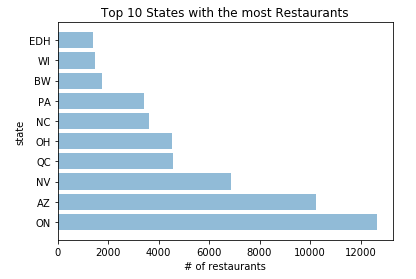
\includegraphics[width=80mm,scale=0.5]{states}
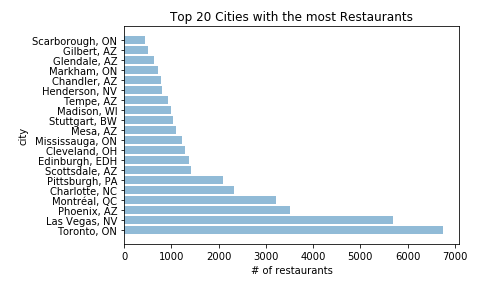
\includegraphics[width=90mm,scale=0.5]{cities}
\end{center}
   
After running some queries and looking at the cities with the most restaurants, we decided to choose Pittsburgh due to the number of restaurants (2089), the significant number of neighborhoods (53), and the variety of cuisines (43 different cuisines). We ended up with these 43 restaurant
cuisines (categories) after filtering out some such as "Burgers", "Pizza" and “Breakfast and Brunch”. We kept all cuisines/categories such as Vietnamese, Asian Fusion, Caribbean, and American (Traditional). Although Phoenix and Las Vegas had more restaurants, Phoenix had no neighborhoods and Las Vegas had fewer neighborhoods. Interestingly enough, Pittsburgh only had 4 restaurants labeled as touristy, so we will look to see if there are particular neighborhoods that are more 'upscale' or 'divey', rather than authentic and touristy.\\

In order to get a better idea of the restaurants within Pittsburgh, we created a simple visualization using the folium library which plots the latitude and longitude of every restaurant on a nice map. Although interesting and useful to implement in order to use it for future visualizations, this doesn't tell us too much other than it appears to be very dense around the middle of the city. Our heat map of restaurant density and the most popular restaurants in Pittsburgh (shown left and right respectively) do show that a lot of the restaurants in the neighborhoods in the center of the city are more popular.

\begin{center}
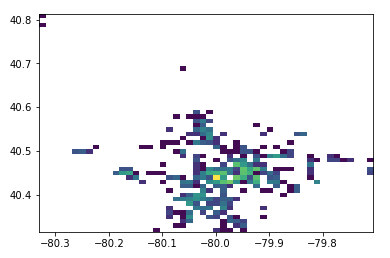
\includegraphics[width=75mm,scale=0.5]{pa_rest_density}
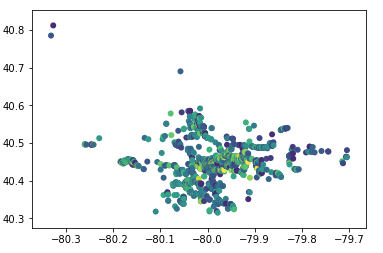
\includegraphics[width=75mm,scale=0.5]{pa_popular_restaurants}
\end{center}

From here, we decided to further explore the Pittsburgh neighborhoods and first discover the top 10 neighborhoods with the most restaurants. Following this, this lead to creating a map of the top 10 neighborhoods with the highest average review count. In other words, we were curious what neighborhoods are the most popular among Yelp reviewers.

\begin{center}
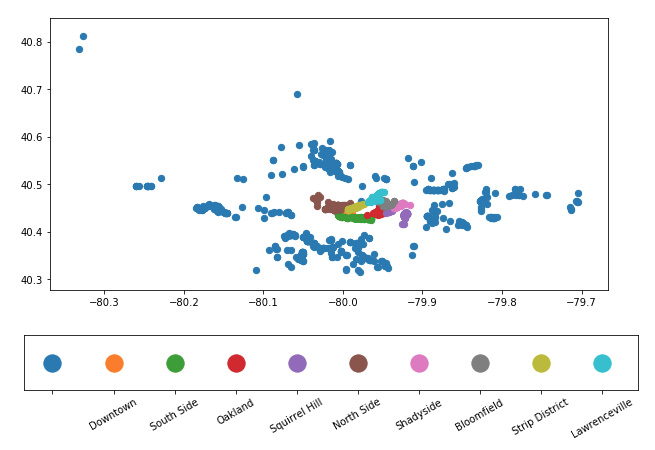
\includegraphics[width=75mm,scale=0.5]{pitts_hoods_most_restaurants}
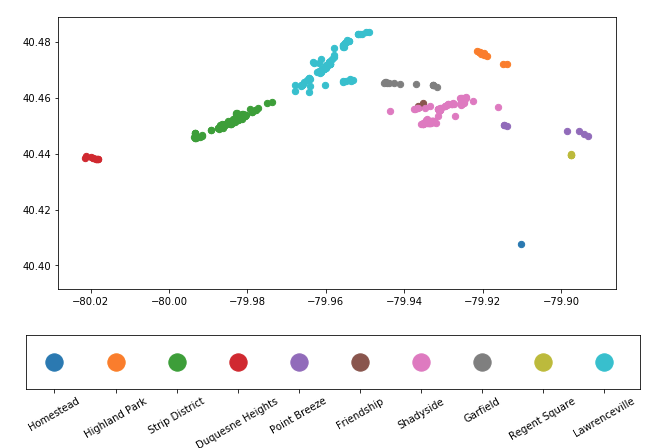
\includegraphics[width=75mm,scale=0.5]{top_10_most_popular_neighborhoods}
\end{center}

To get started on a deeper exploratory analysis of reviews and ratings, we plotted the distribution of the ratings for all the restaurants in Pittsburgh. From the plot we can see that most restaurants have a rating between 3 and 5. The average rating for Pittsburgh restaurants is 3.51. To gain a deeper insight of the data, we plotted the rating distribution of different cuisines. 

\begin{center}
	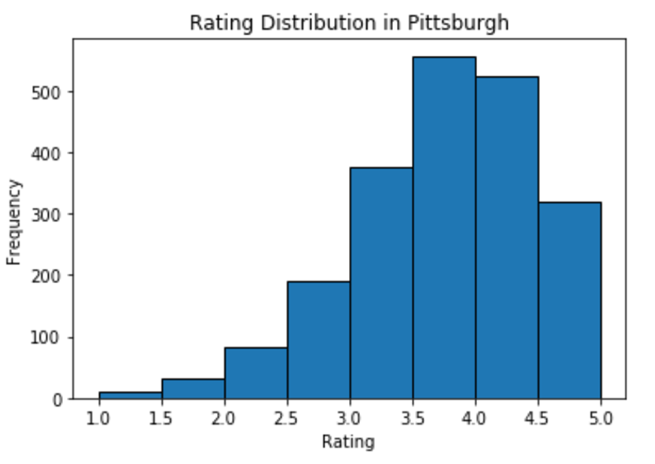
\includegraphics[width=65mm,scale=0.3]{rating_distribution_in_Pittsburgh}
	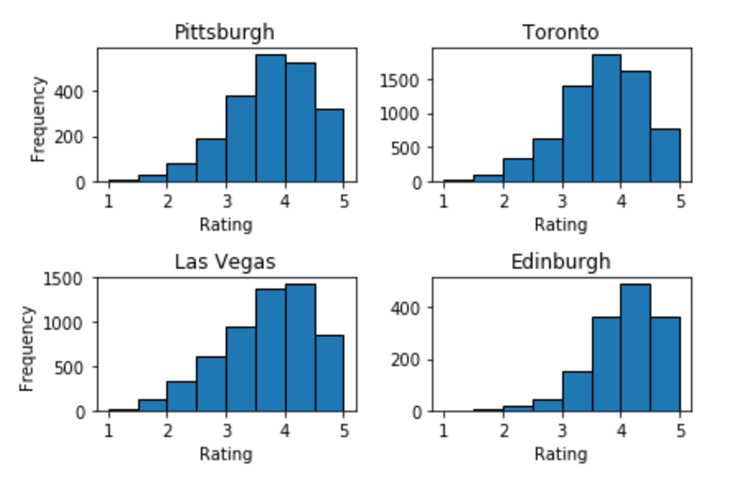
\includegraphics[width=75mm,scale=0.3]{rating_distribution_vs_countries}
\end{center}

Besides looking at the basic distribution, we plotted the relationship between the average number of reviews and rating level using box plot. Our original belief was that we thought better restaurants should receive more reviews. However, the results show us that restaurants with a medium rating acquire more reviews. 

\begin{center}
	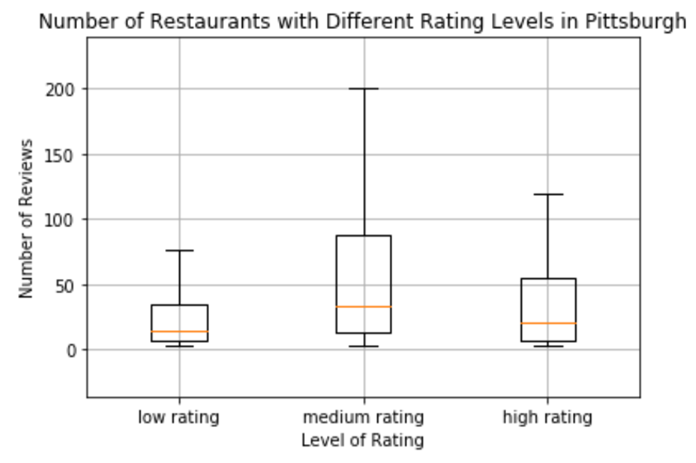
\includegraphics[width=75mm,scale=0.3]{number_of_restaurants_vs_rating_level}
\end{center}

We also explored the relationship between average number of reviews, the average length of review (after tokenization and stemming) and each cuisine. In Pittsburgh in appears that Japanese foods receive the most reviews while Chinese foods receive the least number of reviews. When looking at the length of review, there doesn't appear to be many differences among the variety of cuisines. 

\begin{center}
	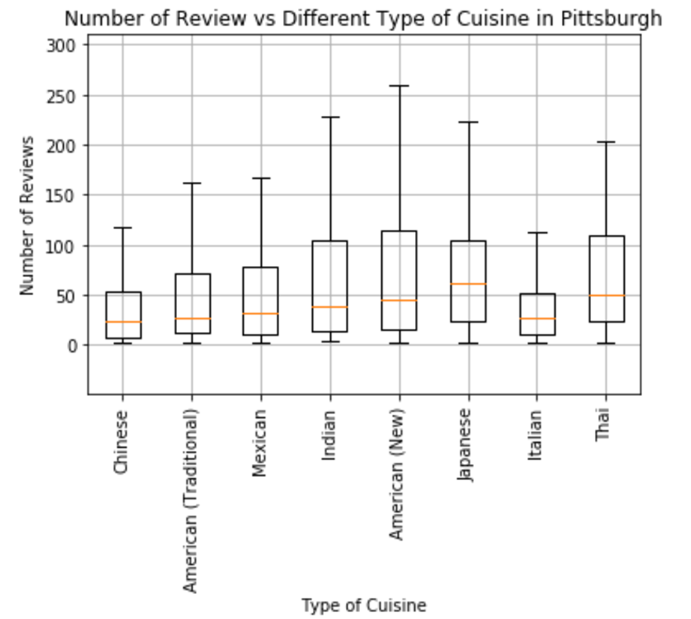
\includegraphics[width=75mm,scale=0.3]{number_of_review_vs_cuisine}
	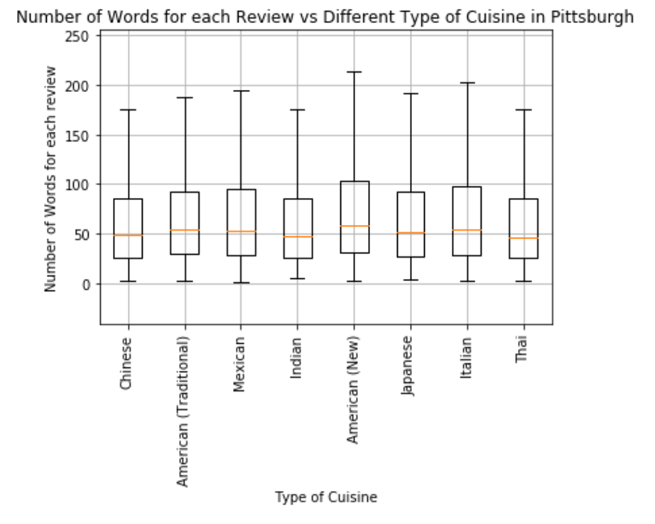
\includegraphics[width=85mm,scale=0.3]{average_review_length}
\end{center}

Furthermore, to get a better sense on how the contents of a review correlate with the rating, we calculated the ratings for one of the restaurant by performing sentiment analysis on the reviews and then comparing the results with the dataset ratings. Through sentiment analysis, we can determine whether the review is positive or negative. We took a sample dataset of all restaurants in Pittsburgh which have more than 200 reviews to assign our own ratings (there are 109 restaurants in Pittsburgh which satisfy our criteria), and computed the average of the values obtained from sentiment analysis of all the reviews (38,785 reviews) of that restaurant. The sentimental analysis is done using PatternAnalyzer in nltk (textblob is built over nltk). We assigned a weight of +5 for a positive review and -5 for a negative review. These newly derived ratings are compared with the ratings in original dataset as shown in the histogram. We can assume that these reviews are more accurate because we are incorporating negative weights to low star reviews.

\begin{center}
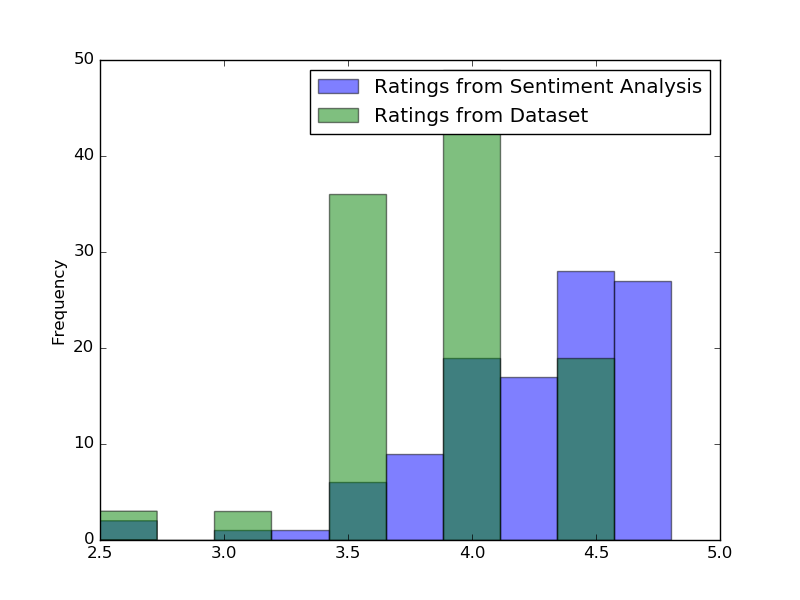
\includegraphics[width=90mm,scale=0.5]{sentimentanalysis}
\end{center}

Next, we extracted the top 50 keywords from positive and negative reviews. Again taking a sample dataset of all restaurants in Pittsburgh that have more than 200 reviews. There are a total of 38,785 reviews. Data processing techniques such as tokenizing, filtering, stemming and filtering the key words from those reviews were performed. We then calculated 50 most frequent keywords from the negative and positive reviews separately. Negative and positive reviews were distinguished using the polarity obtained in the previous step.
The results are very promising. Few keywords such as "great","good","nice","service" came with high frequency in positive reviews where as words like "bad","good","terrible","poor","great" appeared negative reviews. Common words such as "Pittsburgh", "food", "service", and "place" are present in both positive and negative reviews. One important thing to notice is that "good" and "great" appeared in negative reviews too in a sense that customers are complaining how the food isn't that good/great. The high frequencies of words in positive reviews when compared to negative reviews is because of more number of positive reviews in the corpus.

\begin{center}
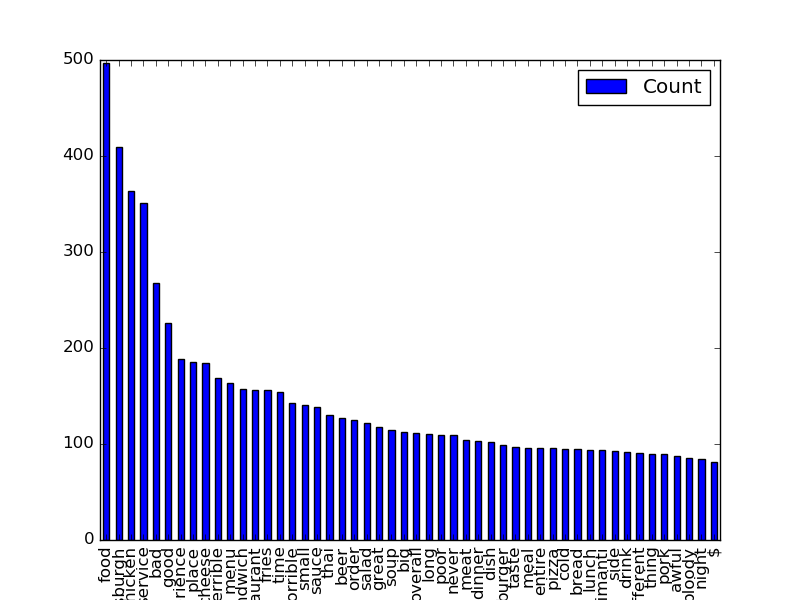
\includegraphics[width=70mm,scale=0.5]{top50_negativereviews}
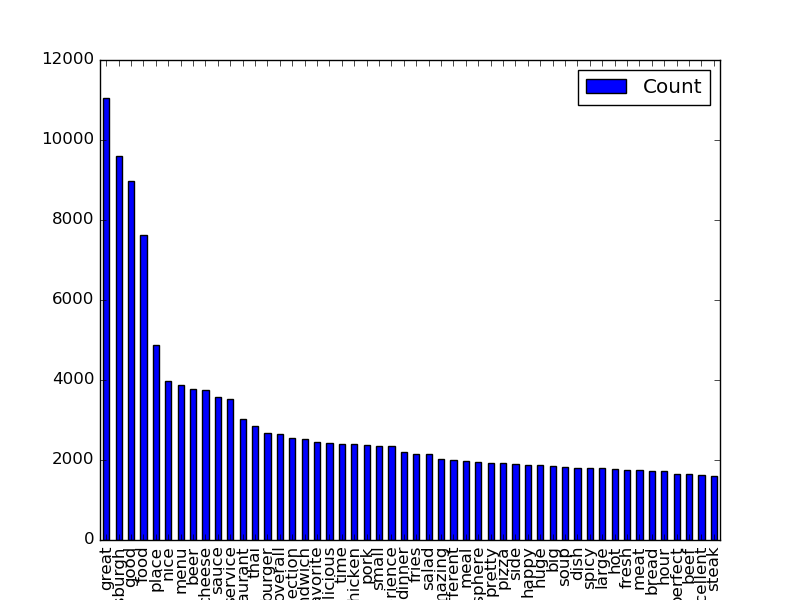
\includegraphics[width=70mm,scale=0.5]{top50_positivereviews}
\end{center}

Although some of our exploratory analysis focused on one city, we expanded our reviews analysis to 4 different cities with the most reviews (Edinburgh, Toronto, Las Vegas, and Pittsburgh), from 3 different countries. The thought here was that there may be differences between different cities such as the service, or people may have different diction. It's possible that the final cluster may be verified by different external evaluation criteria, so we thought it'd be useful to further explore this area. We plotted the differences of rating habits among the 4 cities based on average rating score for each type of cuisine. Edinburgh has the best rating feedback, relatively speaking, while Toronto seems to be lacking Yelper feedback.

\begin{center}
	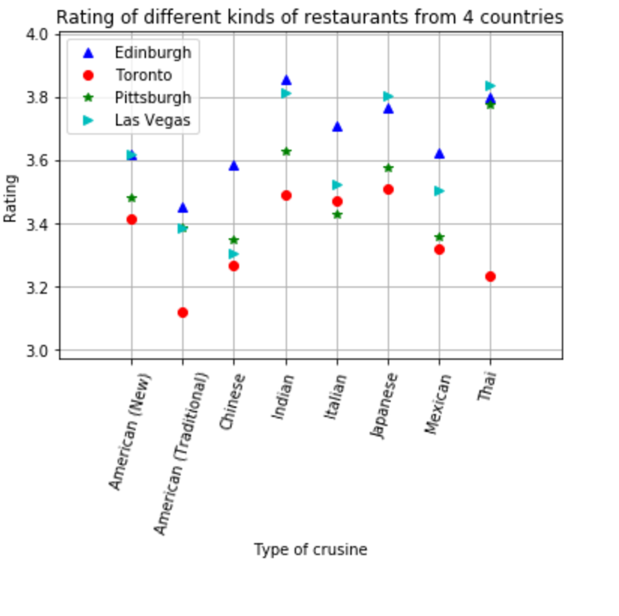
\includegraphics[width=60mm,scale=0.5]{Rating_different_restaurants_countries.png}
\end{center}
\section*{3 Next Steps}
\subsection*{3.1 Algorithms}
In our next phase, we plan on implementing K-Means and Hierarchical clustering algorithms on the Pittsburgh restaurants with respect to cuisines in the neighborhoods. We will perform an analysis on which clustering algorithm produces better results. We'd also like to try clustering by restaurant rating and compare it to it's neighborhood clustering. We will also look to begin the design and implementation of the recommendation system now that we have a much fuller understanding of our data set. 

\subsection*{3.2 Evaluation}
We plan on using evaluation techniques such as cophenetic correlation and proximity correlation comparison. Using purity, we're thinking we can compare the clustering of restaurants by their cuisines to the clustering of the neighborhoods. 

\subsection*{3.3 Modifications}
As see in the report earlier, our sample data was using restaurants that had over 200+ reviews. We plan to reproduce our sentimental analysis for restaurants in Pittsburgh with 30+ reviews since the average number of reviews turned out to be only 50. 


\end{document}
